
%--------------------------------------------------------------------
%                            Preample
%--------------------------------------------------------------------

\documentclass[aspectratio=1610,17pt,utf8]{beamer}

\usepackage[utf8]{inputenc}
\usepackage[T1]{fontenc}
\usepackage[USenglish]{babel}
\usepackage{graphicx} % graphics
\usepackage{mathabx}
\usepackage{mathpazo}
\usepackage{eulervm}

\usepackage{xcolor}

\pagenumbering{arabic}

\newcommand{\mainframe}[1]{\color{blue} 
\includegraphics[width=.05\textwidth]{figures/aau.png} #1\\\color{black}\hrule}

\newcommand{\regularframe}[1]{\color{black}
\includegraphics[width=.05\textwidth]{figures/aau.png} #1\\\hrule}

\addtobeamertemplate{navigation symbols}{}{
    \usebeamerfont{footline}
    \usebeamercolor[fg]{footline}
    \hspace{1em}
    \insertframenumber/\inserttotalframenumber
}

% title slide definition
\title[DS]{Distributed Systems}
\subtitle{Exam}
\author[Thomas Møller Jensen]{Thomas Møller Jensen}
\institute[Institute of Computer Science]
{
  Aalborg University\\
}

%--------------------------------------------------------------------
%                            Titlepage
%--------------------------------------------------------------------

\begin{document}

%-------------------------------------------------------------------
%                            Content
%-------------------------------------------------------------------
%                 Distributed Mutual Exclusion
%-------------------------------------------------------------------

\begin{frame}{\mainframe{Distributed Mutual Exclusion}}
    What is a mutex? Kinda a Lock for distributed systems \ldots

    In a distributed system a mutex is for locking a shared resource in a network, traditionally in a program, a lock would be enough to handle concurrent writes/reads, but when the communication is expensive, locking the resource is harder to do.
\end{frame}

% A mutual exclusion means that a shared resource between processes should be coordinated between processes in some way. For this there are multiple algorithms that can ensure a network can reach mutual exclusion. They have their advantages and disadvantages that i will discuss in this presentation

\begin{frame}{\regularframe{Mutex Algorithms}}
    \section{Mutex algorithms}
    \begin{itemize}
        \item Centralized Algorithm
        \item Token Ring Algorithm
        \item Ricart and Agrawala's algorithm
        \item Maekawas algorithm
    \end{itemize}
\end{frame}

% The centralized algorithm is an algorithm where a centralized server will handle whether a process can access the critical resource in a network.
% This is a very simple architecture, and its implementation is simple, but it also has a huge flaw that any failures at the centralized server will result in a full system failure. This is bad.

\begin{frame}{\regularframe{Centralized algortihm}}
    \begin{minipage}{.45\textwidth}
        \begin{figure}
            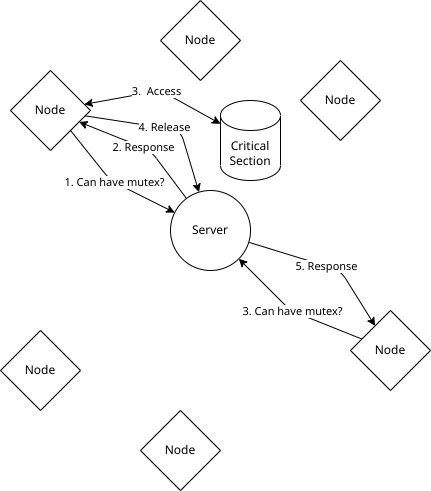
\includegraphics[width=\textwidth]{figures/1-mutex.png}
        \end{figure}
    \end{minipage}
    \begin{minipage}{.5\textwidth}
        \tiny{All three nodes highlighted are points of failure.}
    \end{minipage}
\end{frame}

% This is the token ring algorithm, the idea here is to remove the centralized server from the system, essentially making the system completely decentralized. Here the devices are communicating a token to each other which signifies that that process is allowed to access the critical section. One of the big advantages of this algorithm is how much each node can communicate with the critical section. once it has the token, it can communicate all it wants with the critical section until it transmits the token to the next device.
% The disadvantage of such a system is that if one node fails the whole system fails.

\begin{frame}{\regularframe{Token Ring Algorithm}}
    \begin{minipage}{.45\textwidth}
        \begin{figure}
            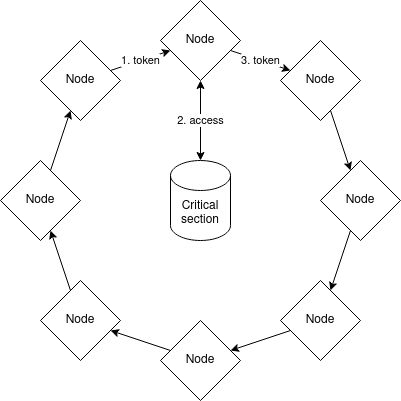
\includegraphics[width=\textwidth]{figures/1-token.png}
        \end{figure}
    \end{minipage}
    \begin{minipage}{.5\textwidth}
        \tiny{All nodes are points of failure at any given time.}
    \end{minipage}
\end{frame}

% The ricart and agrawala's algorithm is one where each of the nodes keeps track of whether a node is in the critical section at any time.
% This is useful as if multicast is efficient, then access is granted swiftly while any node wishing to enter doesn't have to communicate, it would know if anyone is accessing the critical section
% Once again the disadvantage is that one node failing means the whole system fails

\begin{frame}{\regularframe{Ricart and Agrawala's algorithm}}
    \begin{minipage}{.45\textwidth}
        \begin{figure}
            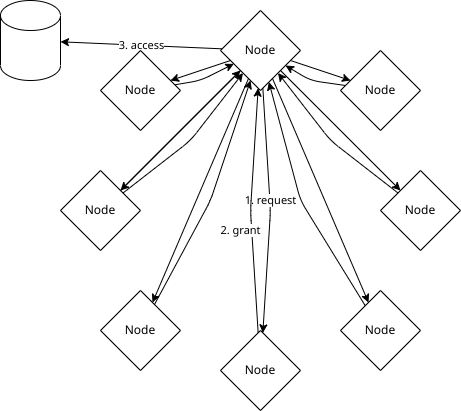
\includegraphics[width=\textwidth]{figures/1-ricart-agrawala.png}
        \end{figure}
    \end{minipage}
    \begin{minipage}{.5\textwidth}
        \tiny{All requests are multicast.\\There is a 4th step where a release is multicast to all nodes as well.\\All nodes are points of failure at any given time.}
    \end{minipage}
\end{frame}

% This algorithm is similar to ricart and agrawala, but instead of asking each node in the network, it only has to ask a small subset of the network.
% This can be 

\begin{frame}{\regularframe{Maekawas algorithm}}
    \begin{minipage}{.45\textwidth}
        \begin{figure}
            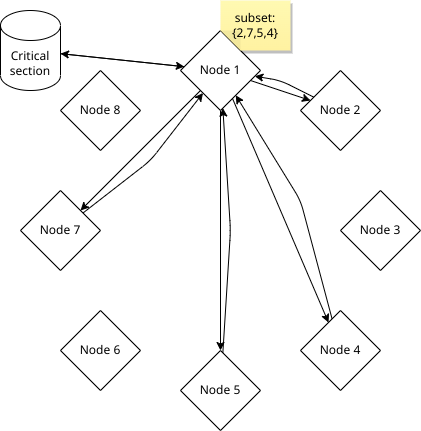
\includegraphics[width=\textwidth]{figures/1-maekawa.png}
        \end{figure}
    \end{minipage}
    \begin{minipage}{.5\textwidth}
        \tiny{Very similar to Ricart and Agrawala, but only nodes in the subset failing will result in a particular node to fail. If you're a bit smart about choosing the subsets this can be minimized.}
    
        \begin{table}
            \begin{tabular}{|c|c|c|c|c|}\hline
                n & n & n & n & n \\\hline
                n & $p_1$ & n & n & n \\\hline
                n & n & n & n & n \\\hline
                n & n & n & $p_2(f)$ & n \\\hline
                n & n & n & n & n \\\hline
            \end{tabular}
        \end{table}
    
    \end{minipage}

\end{frame}

\begin{frame}{\regularframe{Performance}}
    Bandwidth means Entry and Exit potential. This means how many times an acces can happen per messages.\\
    Token ring is infinite because the node itself chooses when to send the token.\\
    Ricart and Agrawala's algorithm has a bandwidth of 1+n-1 if it can do multicast in hardware, otherwise its n-1+n-1, as it will now have to unicast to everyone.
    \tiny{\begin{table}
        \begin{tabular}{|c|c|c|c|c|}
            \hline
            Algorithm & Entry & Exit & sync & Bandwidth \\\hline
            Centralized & 2 & 1 & 2 & 2 / 1 \\\hline
            Token Ring & a:n/2 w:n-1 & 1 & a:n/2 w:n-1 & $\infty$ / 1 \\\hline
            R + A & 2 & 2 & 1 & 1+n-1 or n-1+n-1 / n-1 \\\hline
            maekawa & 2 & 1 & 2 & $4 \sqrt{n}-2$ / $2 \sqrt{n}-1$ \\\hline
        \end{tabular}
    \end{table}}
\end{frame}
%-------------------------------------------------------------------
%                 Multicast/Group Communication
%-------------------------------------------------------------------

\begin{frame}{\mainframe{Multicast/Group Communication}}

    \begin{figure}
        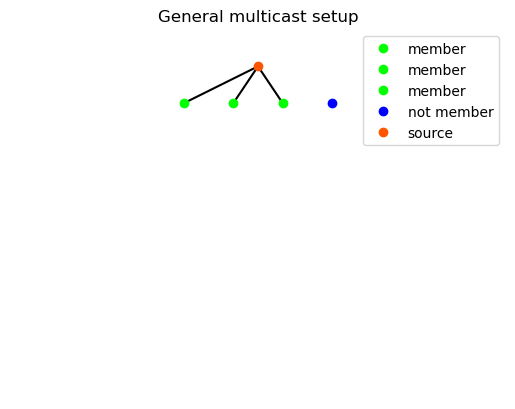
\includegraphics[width=1\textwidth]{figures/2-multicast-group.png}
    \end{figure}
\end{frame}

\begin{frame}{\regularframe{IP Multicast - Hardware Support}}
    Uses a protocol called IGMP

    If there's hardware support, the sender transmits one message and the intermediary devices will determine how many devices it will transmit the message to.\\
    If there is not hardware support, then the sender will have to unicast many messages at once to its receivers instead.
\end{frame}

\begin{frame}{\regularframe{IP Multicast - Problems}}
    Out of order delivery, this can happen due to changes in routing. Consider a network with a slow and a fast intermediary node as two independant routes, if the sender sends a message through the slow node to the reciver followed by a message through the fast node, then the receiver might receive the second message before the first.
\end{frame}

\begin{frame}{\regularframe{IP Reliable Multicast}}
    \begin{itemize}
        \item Trading efficiency for reliability
        \item ACKs - increases time complexity to $O(n^2)$
    \end{itemize}
\end{frame}

\begin{frame}{\regularframe{FIFO! First In - First Out Multicast}}
    Respects sequence numbers\\
    IP Multicast is FIFO

\end{frame}

\begin{frame}{\regularframe{Total Ordering: Using a Sequencer}}
    Messages should arrive in the same order as they were sent\\
    A central server handles giving each message a sequence number.\\
    Single point of failure
    \begin{figure}
        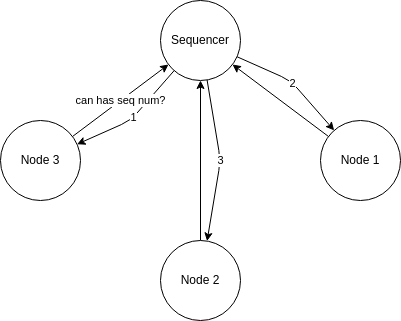
\includegraphics[width=.3\textwidth]{figures/sequencer.drawio.png}
    \end{figure}
\end{frame}

\begin{frame}{\regularframe{Causal Ordering}}
    Generally, causal ordering means that the events in a network does not depend on a future event, this is usually realized using lamport clocks.\\
    A lamport clock is simply a clock that increments before each event on a node, and is synchronized at the receiver.


\end{frame}

\begin{frame}{\regularframe{Clocks for ordering}}
    \begin{figure}
        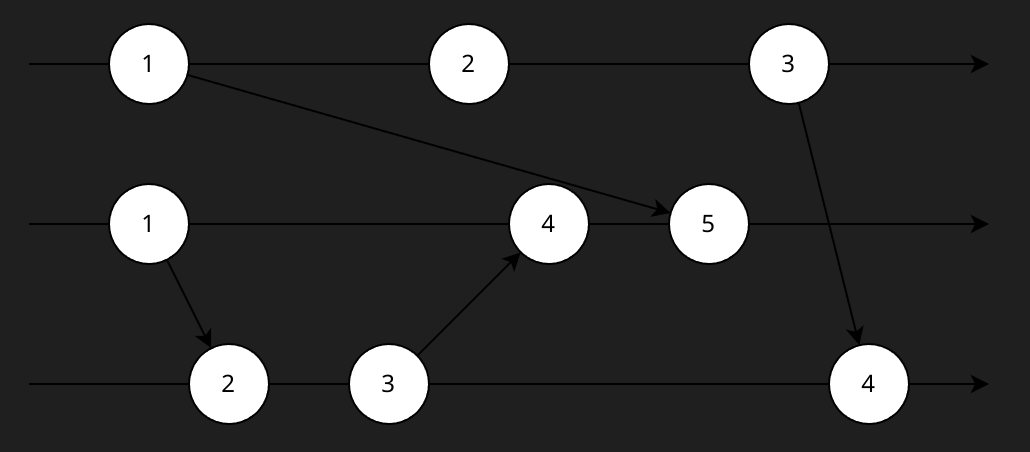
\includegraphics[width=.5\textwidth]{figures/2-lamport.png}
    \end{figure}
    \begin{figure}
        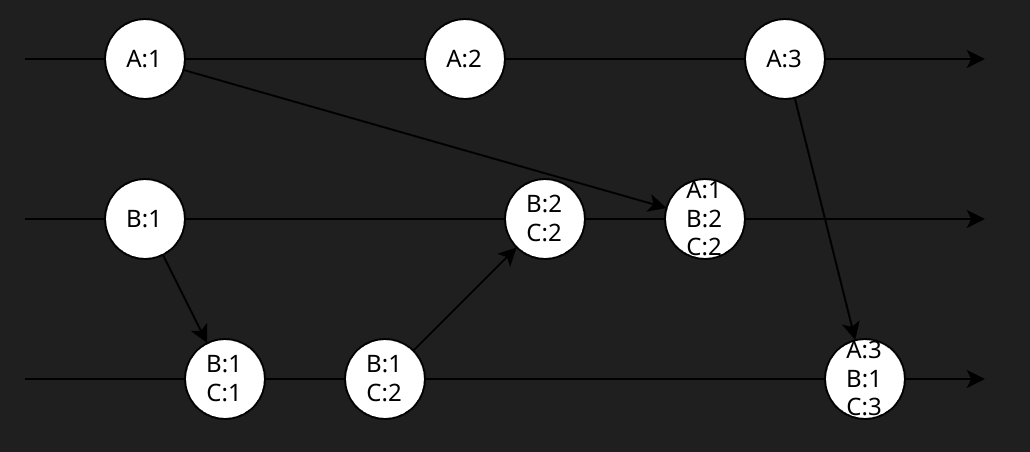
\includegraphics[width=.5\textwidth]{figures/2-vector.png}
    \end{figure}
\end{frame}



%-------------------------------------------------------------------
%                     Consensus Protocols
%-------------------------------------------------------------------

\begin{frame}{\mainframe{Consensus Protocols}}
    The idea is to make sure processes agree\\
    Synchronous Consensus Algorithm\\
    Byzantine Generals Algorithm\\
    Phase-King Algorithm
\end{frame}


\begin{frame}{\regularframe{Byzantine faults}}
    The armies example, one half retreats, one attacks.\\
    Two different descisions was made, this is an error\\
    Byzantine failures are by extension when the whole system fails due to a byzantine fault.
\end{frame}

\begin{frame}{\regularframe{Correct Processes}}
    A correct process is a process that is operating as expected. Closely tied with byzantine faults, if a process has a byzantine fault, then it is no longer a correct process.
\end{frame}

\begin{frame}{\regularframe{Synchronous Consensus Algorithm}}
    f-resilience, f processes may fail
    \begin{itemize}
        \item initially multicast your value
        \item do f+1 rounds
        \item in each round, process received messages, record how many times each unique value is received
        \item multicast again
    \end{itemize}
\end{frame}

\begin{frame}{\regularframe{Byzantine Generals}}
    > you have commanders and lieutenants, its kinda like master and slaves in other systems, the commander says a value, and the lieutenants take this value as the correct value.\\
    > In this system, if the commander is not correct, it results in a failure.\\
    > when the value is received from the commander, the lieutenants multicast their received value and id, then the majority value is chosen at each process.
\end{frame}

\begin{frame}{\regularframe{Phase-King algorithm}}
    This algorithm can be seen easier in my implementation\\
    > generals only work for f = 1, and can be optimized\\
    f+1 phases\\
    > in each phase, all processes start by transmitting their value, if the most frequest received value is from more than half of the processes, use that value\\
    > the king is elected, process with id k is elected at phase k\\
    > the purpose of the king is to send a tie breaker if two processes share the same count of values.
\end{frame}

\begin{frame}{\regularframe{Paxos}}
    PAXOS is a consensus protocol used in Chubby, in this algorithm 3 types of nodes are defined:\\
    > Proposer\\
    > Accepter\\
    > Learner\\
    Proposers say a value, accepters accept that value and agree on the majority amongst themselves. Learners takes proposed values.
\end{frame}

%-------------------------------------------------------------------
%                 Replication and Consistency
%-------------------------------------------------------------------

\begin{frame}{\mainframe{Replication and Consistency}}
    Goal of replication:\\
    > To tolerate failures\\
    > High availability\\
    > More affordable to scale out\\
    > caching is replication
\end{frame}

\begin{frame}{\regularframe{Replication}}
    \begin{minipage}{.45\textwidth}
        \begin{figure}
            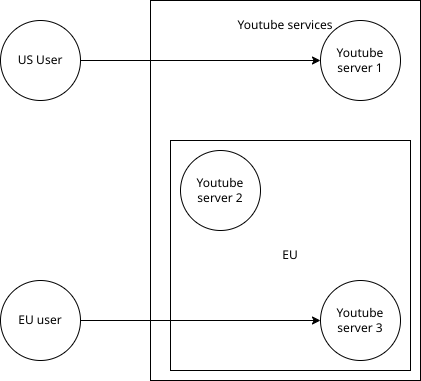
\includegraphics[width=\textwidth]{figures/4-replication.drawio.png}
        \end{figure}
    \end{minipage}
    \begin{minipage}{.5\textwidth}
        > each server has videos cached\\
        > if server 3 goes down, the EU user can use server 2
    \end{minipage}
\end{frame}

\begin{frame}{\regularframe{Passive Replication}}
    > One primary node, all other nodes are backup
\end{frame}

\begin{frame}{\regularframe{Consistency}}
    Youtube: like count is consistent while views are relaxed consistency

    What if user A and user B of a bank system adds money at the same time? all nodes has to agree on one value

\end{frame}

\begin{frame}{\regularframe{Sequential consistency}}
    Follows lamport clocks, the system should follow the order in which the events arrive.
\end{frame}

%-------------------------------------------------------------------
%                     Distributed Storage
%-------------------------------------------------------------------

\begin{frame}{\mainframe{Distributed Storage}}
    Cheaper/more efficient to scale out storage rather than scale up.\\
    imagine a large database which gets overloaded with queries, its a better idea to have multiple servers handle the load.\\
    Imagine if youtube had all videos on one system, it would perform better if you had two systems and every second video is on the other system.
\end{frame}

\begin{frame}{\regularframe{Big Data Storage}}
    Often one system can't handle the amount of data stored \\
    Google/facebooks large amounts of data
\end{frame}

\begin{frame}{\regularframe{Chubby}}
    uses distributed consensus protocol PAXOS\\
    Not designed for frequent locking and unlocking, some devices may hold a lock for days.\\
    Clients elects a master node, the master node has the role of writing the database while also making sure that any replicas of it also writes the same data.
\end{frame}
\begin{frame}{\regularframe{Paxos}}
    PAXOS is a consensus protocol used in Chubby, in this algorithm 3 types of nodes are defined:\\
    > Proposer\\
    > Accepter\\
    > Learner\\
    Proposers say a value, accepters accept that value and agree on the majority amongst themselves. Learners takes proposed values.
\end{frame}

\begin{frame}{\regularframe{GFS Filesystem}}
    A filesystem designed to have direct access to files across a cluster of distributed storage nodes.\\
    One master node to manage the systems.\\
    Master node prevents single point of failure by maintaining extra nodes for replication.
\end{frame}

%-------------------------------------------------------------------
%                     Big Data Analytics
%-------------------------------------------------------------------

\begin{frame}{\mainframe{Big Data Analytics}}
    Why? Lots of unstructured data could be processed\\
    Not suited for traditional databases\\
\end{frame}

\begin{frame}{\regularframe{Map Reduce}}
    It is a method to take large chunks of data, split them and process them in parallel on distributed nodes, and finally aggregating them.\\
    Functional programming style data processing:\\
    Map: maps a key to generate some value\\
    Reduce: any equivalent key is reduced together with similar keys to single values.\\
\end{frame}

\begin{frame}{\regularframe{Map Reduce}}
    \begin{figure}
        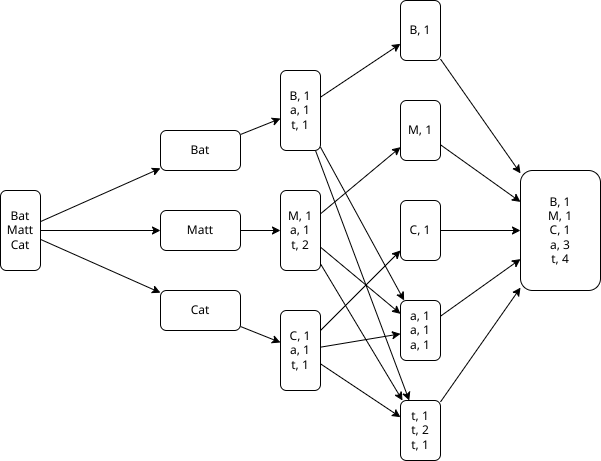
\includegraphics[width=.6\textwidth]{figures/mapreduce.drawio.png}
    \end{figure}
\end{frame}

\begin{frame}{\regularframe{Fault Tolerance}}
    workers are pinged by master node (first in previous diagram)\\
    master is a single point of failure
\end{frame}

\begin{frame}{\regularframe{Spark (RDD)}}
    Another way to process big data\\
    Data is ordered in \texttt{Resilient Distributed Database}s. an immutable data structure that can be operated on in parallel.\\

\end{frame}

%-------------------------------------------------------------------
%                         Blockchains
%-------------------------------------------------------------------

\begin{frame}{\mainframe{Blockchains}}
    Blockchains are Peer-To-Peer Networks
    Hashing\\
    > Compare a hash representing data instead of comparing data\\
    > Make hashes for portions of data if its too large
\end{frame}

\begin{frame}{\regularframe{The Three Algorithms}}
    generateKeys\\
    > Generate private and public keys\\
    sign\\
    > Compute a hash based on the secret key\\
    verify\\
    > Check if the message and hash matches based on the public key\\
    Example: passwordless ssh
\end{frame}

\begin{frame}{\regularframe{The Blockchain}}
    each block is identified by a hash\\
    A tamper proof linked list, $HP_2$ depends on $HP_1$\\
    Essentially a decentralized database\\
    A hash pointer is like a tuple of the address for the next block and a hash of the current block
    \begin{figure}
        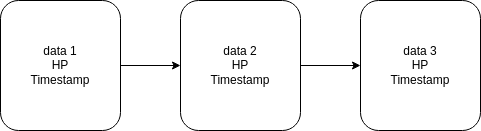
\includegraphics[width=\textwidth]{figures/blockchain.drawio.png}
    \end{figure}
\end{frame}

\begin{frame}{\regularframe{Example: Bitcoin/Crypto}}
    ownership of a block of data, a coin is determined by the owner signing a block against their private keys\\
    NFT's are also data on a blockchain, so ownership of these are signed in a similar way.
\end{frame}

\begin{frame}{\regularframe{Merkle Trees}}
    \begin{figure}
        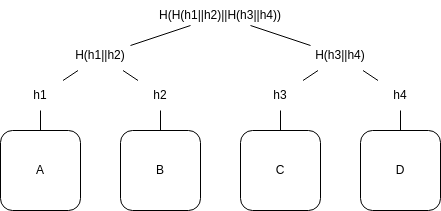
\includegraphics[width=\textwidth]{figures/merkle.drawio.png}
    \end{figure}
\end{frame}

%-------------------------------------------------------------------
%                  Peer-to-Peer Networking
%-------------------------------------------------------------------

\begin{frame}{\mainframe{Peer-to-Peer Networking}}
    Overlay networks and underlying network\\
    Three types of peer-to-peer networks\\
    > Unstructured\\
    > Structured\\
    > Centralized
\end{frame}

\begin{frame}{\regularframe{Overlay Networks}}
    This network is like an abstraction of the underlying architecture.\\
    Green: overlay, Yellow underlying network
    \begin{figure}
        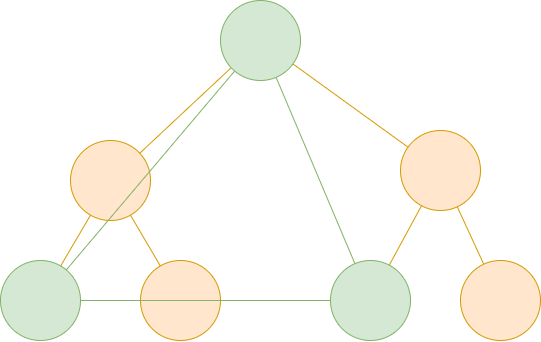
\includegraphics[width=.55\textwidth]{figures/overlay-networks.drawio.png}
    \end{figure}
\end{frame}

\begin{frame}{\regularframe{Unstructured P2P Networks}}
    No central server\\
    No structure in the overlay network\\
    Devices come and go from the network very frequently\\
    very slow search due to flooding
\end{frame}

\begin{frame}{\regularframe{Structured P2P Networks}}
    Can be structured according to rings.\\
    in a ring, a node would maintain pointers to the next node and previous node\\
    if a node wants to join, it'll first contact an arbitrary node, that will contact around the ring until the previous node can tell the new node who its next is, connection between the new and next node is established and finally the new node can join.
\end{frame}

\begin{frame}{\regularframe{Centralized P2P Networks}}
    Structured around a centralized server\\
    Centralized server has no data, it will just return the physically closest other client that has the data
\end{frame}

\begin{frame}{\regularframe{Advantages/Disadvantages}}
    Advantages\\
    > Inherently scalable\\
    > Inherently Fault Tolerant\\
    Disadvantages\\
    > Security\\
    > Backups are hard
\end{frame}

%-------------------------------------------------------------------
%              Internet of Things and Routing
%-------------------------------------------------------------------

\begin{frame}{\mainframe{Internet of Things and Routing}}
    Terminology:\\
    > Embedded Systems, WSN, CPS, IoT\\
    Low power, Real time, etc...\\
\end{frame}

\begin{frame}{\regularframe{Wireless Sensor Networks}}
    monitoring\\

    Example: P7 Project\\
    First draft project: Deep Sleep and energy saving\\
    \begin{figure}
        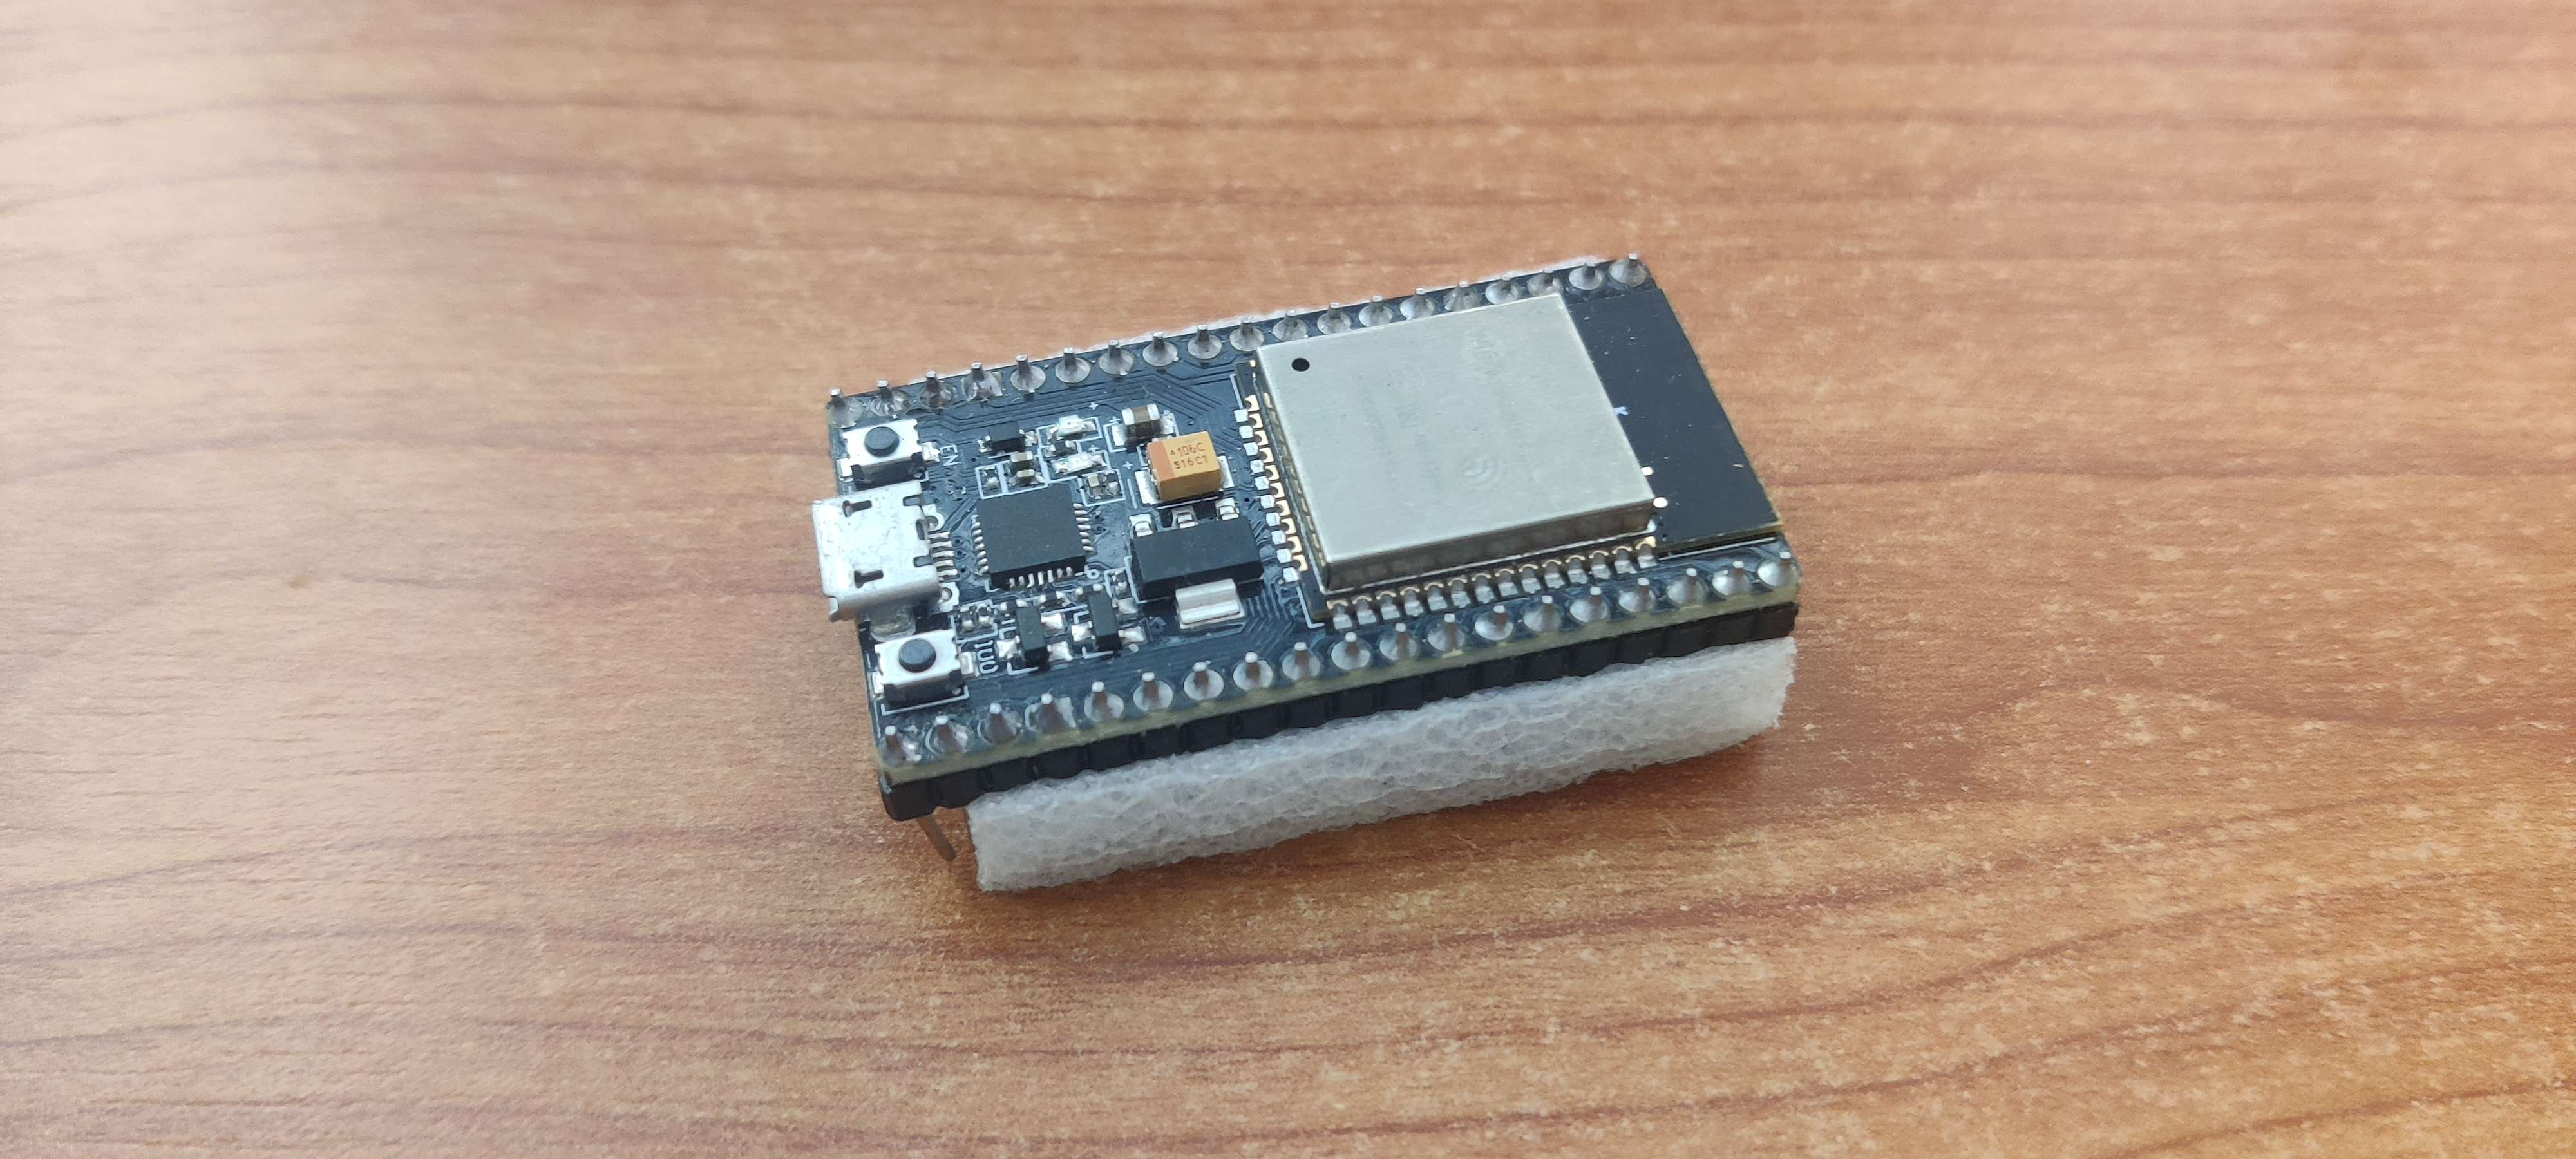
\includegraphics[width=.8\textwidth]{figures/esp32.jpg}
    \end{figure}
\end{frame}

\begin{frame}{\regularframe{Typical Protocols in WSN/IoT}}
    WiFi WLAN\\
    Bluetooth PAN\\
    Others? ZigBee, LoRA, CSMA, ...\\
    Example: P1 LoRA wireless sensors\\
    \begin{figure}
        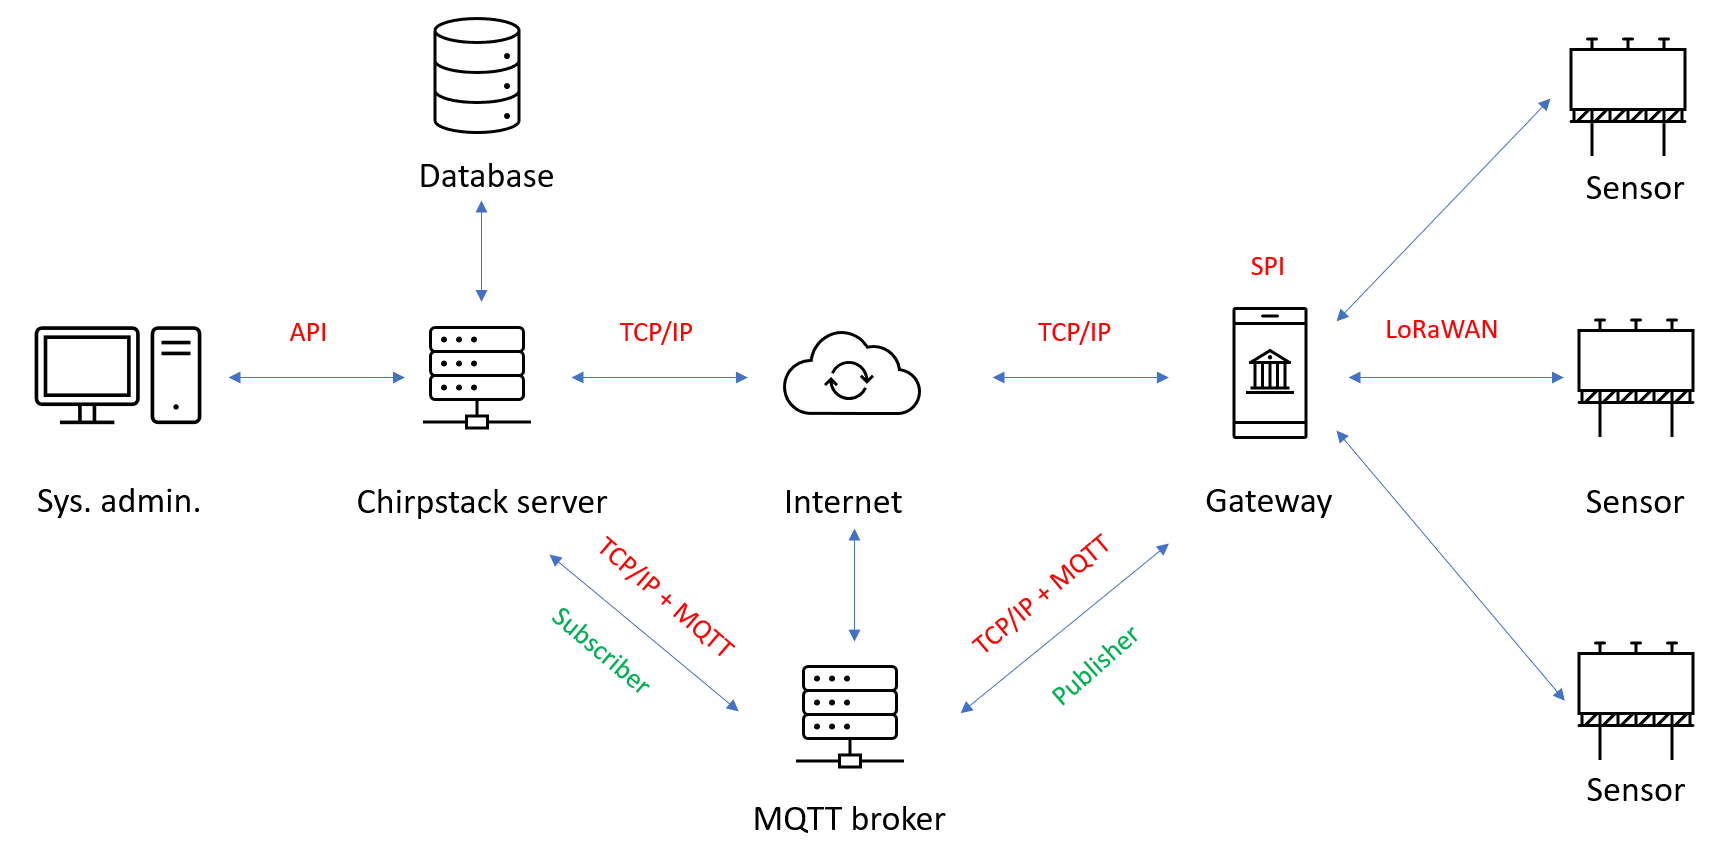
\includegraphics[width=.6\textwidth]{figures/system_oversigt.png}
    \end{figure}
\end{frame}

\begin{frame}{\regularframe{CSMA}}
    MAC Layer protocol\\
    You can compare this protocol with TDMA (Time Division Multiple Access) where the channel is split into time slots for each user, while CSMA listens for concurrent transmissions before transmitting.\\
    > Many devices waiting on a channel to be ready is prone to collisions\\
    > Collision Avoidance % find shit from NDS
\end{frame}

\begin{frame}{\regularframe{Route Discovery DSR}}
    Flooding\\
    \begin{figure}
        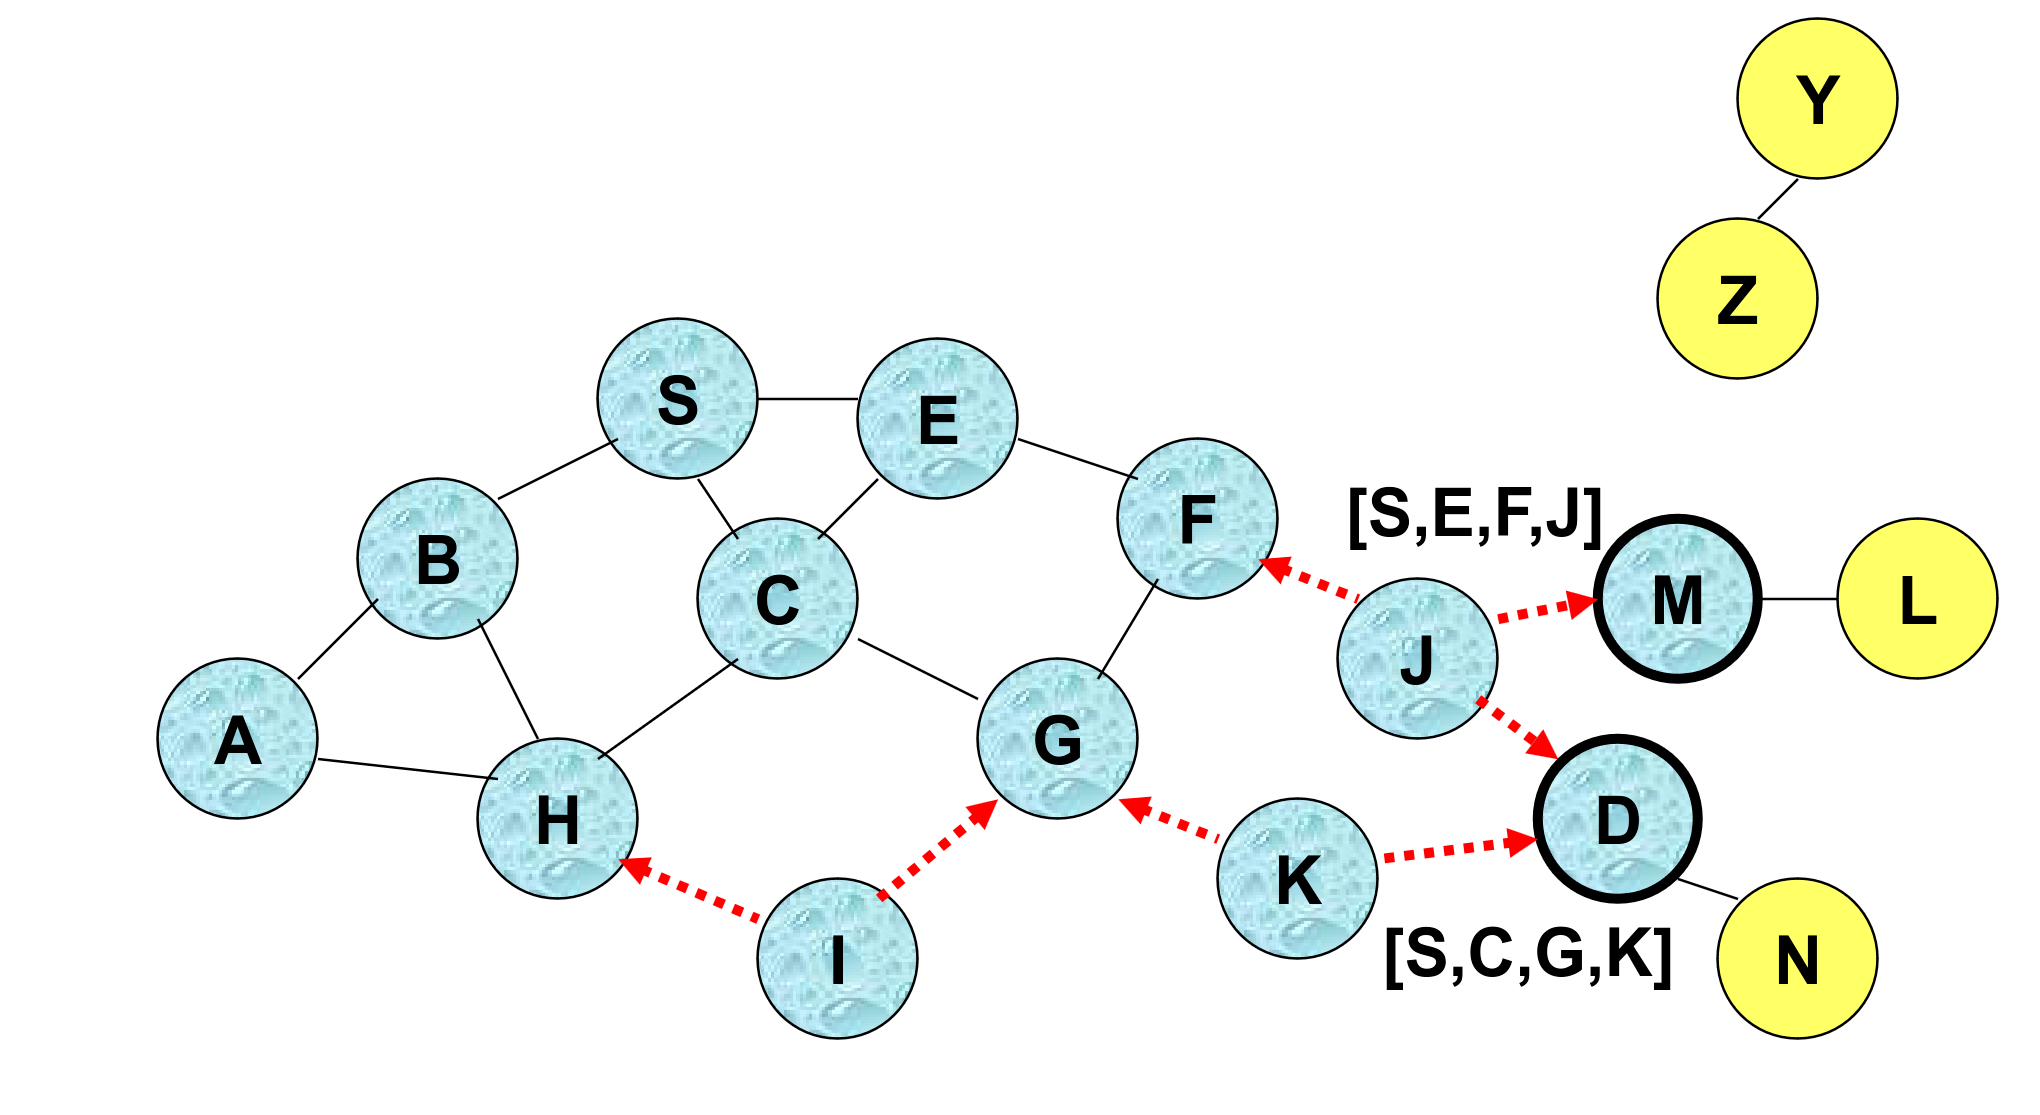
\includegraphics[width=.9\textwidth]{figures/route-discovery.png}
    \end{figure}
\end{frame}

\end{document}